\chapter{Lecture Notes}

\section{05.09.24 - Meassurements}

\subsection{Agenda}
The agenda of this lecture is:
\begin{highlight}
    \begin{itemize}
        \item Monitoring a food process – why?
        \subitem * Variability of a process
        \subitem * Type of variations
        \item Characterization of a process by measuring
        \item Classification of process analyzers/sensors
        \item Correlations between measurements
    \end{itemize}
\end{highlight}

\subsection{Variability}
Variability in the food industry can take many shapes, such as:
\begin{highlight}
    \begin{itemize}
        \item Raw materials
        \item Equipment
        \item Operators
        \item Environment
    \end{itemize}
\end{highlight}

These variables holds a big influence on the final product, and therefore it is important to monitor the process to ensure a consistent product. Therefore the overall food quality is correlated to the variability of the process.

\subsubsection*{Raw materials}
The quality of ingredients can vary due to factors like soil quality, weather conditions, and transportation. This directly impacts the final product's consistency and taste.

\subsubsection*{Equipment}
Variations in equipment calibration or wear and tear can lead to inconsistencies in processing, such as uneven cooking or mixing.

\subsubsection*{Operators}  
Human error or differences in skill levels among workers can introduce variability in tasks like sorting, measuring, and packaging.

\subsubsection*{Environment}
Factors like temperature, humidity, and cleanliness of the production facility can also contribute to variability in food quality.

\subsection{What is quality?}
By understanding and monitoring these variables, food manufacturers can identify and address sources of variability to improve product quality and consistency.

Quality can be defined as the degree of excellence of something. In the context of food production, quality can refer to the characteristics of a product that meet or exceed customer expectations. This includes factors like taste, appearance, texture, and safety. \textbf{BUT} Quality can also refer to the consistency and reliability of a product, meaning that it meets the same standards every time it is produced.

Here are listed some examples of quality attributes in food production:

\begin{highlight}
    \begin{itemize}
        \item \textbf{Performance} (Will the product do the intended job?)
        \item \textbf{Reliability} (How often does the product fail?)
        \item \textbf{Durability} (How long does the product last?)
        \item \textbf{Serviceability} (How easy is it to repair the product?)
        \item \textbf{Aesthetics} (What does the product look like?)
        \item \textbf{Features} (What does the product do?)
        \item \textbf{Perceived Quality} (What is the reputation of the company or its product?)
        \item \textbf{Conformance to Standards} (Is the product made exactly as the designer intended?)
    \end{itemize}
\end{highlight}

This shows that quality is a multifaceted concept that encompasses many different aspects of a product or service.

A good rule of thumbs is that with a increasing variability, the quality of the product decreases. This is depicted in figure \ref{fig:qualVSvar}.
\begin{figure}[h]
    \centering
    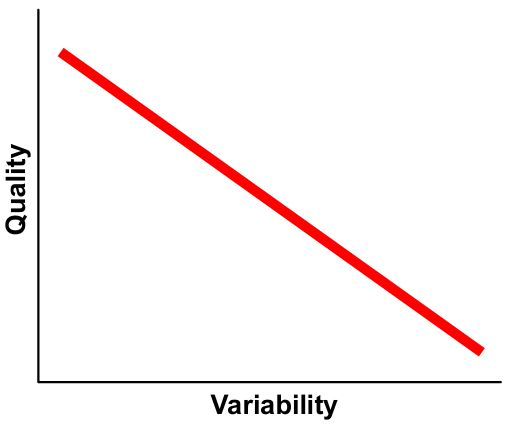
\includegraphics[width=0.35\textwidth]{Figures/qualVSvar.JPG}
    \caption{A picture of the correlation between variability and quality}
    \label{fig:qualVSvar}
\end{figure}

\vspace{2\baselineskip}

A definition of \textit{Quality Improvement} is the reduction of variability in processes and products. The next part of the lecture will focus on how to measure and control this variability.

\subsection{Variability}    
Variability is inherent in every process, and it can be classified into two main types: "Natural" or common cause variation and "special" or assignable cause variation. In common the variability can be measured. 
\subsubsection{Statistical Process Control (SPC)}
This is the variability which is also called the common cause variation. This is the variability that is inherent in the process itself, and it is caused by factors that are part of the normal operation of the process. This type of variation is predictable and can be managed through statistical process control methods. This can affect virtually every production process, from manufacturing to service industries.The SPC follows a probability distribution, so e.g. mean and standard deviation can be calculated for at normal distribution. If the distribution of outputs falls within acceptable limits, the process is said to be in control. If the distribution falls outside of these limits, the process is considered out of control and corrective action is needed. The objectives is to check if we are in control or otherwise act on it.

\subsubsection{Natural Variations}
Natural variations, also called common cause variations, are inherent in the process and are caused by factors that are part of the normal operation of the process (Examples can be poor process design, inadequate equipment and procedure). These variations are predictable and can be managed through statistical process control methods. For example, the temperature of an oven may naturally fluctuate within a certain range during baking, leading to variations in the final product. The natural variations may be identified by the operators, but only management can eliminate common cause variations.

\subsubsection{Assignable Variations}
This is generally caused by factors that are not part of the normal operation of the process, and they are often due to human error, equipment failure, or other external factors.Because of this, the variations can often be traced back to a specific reason. These variations are unpredictable and can be more difficult to manage than common cause variations. For example, if a machine malfunctions during production, it can lead to defects in the final product. Assignable variations are also known as special cause variations, and they require immediate corrective action to bring the process back into control (Eliminate the bad cause and incorporate the "good" cause).




\section{05.09.24 - ISO 22000:2018 - A food safety management system standard}


\textbf{Management} is the way in which an organization manages the inter-related parts of its business in order to achieve its objectives.
There were given a link which can be used to get more information:
https://www.iso.org/management-system-standards.html
(5/9/2018)

\textbf{Standard} (= scheme), this describes the set of rules/requirements on which the system of an organization are based…

Here are some examples of Food Safety Management System Standards:
\begin{highlight}
    \begin{itemize}
        \item BRC Global standard – Food
        \item IFS
        \item SQF
        \item ISO 22000
        \item FSSC 22000
        \item For more examples, see QM-textbook, pp. 7-12
    \end{itemize}
\end{highlight}

\subsection{Deming Circle}
The Deming Circle, also known as the PDCA Cycle (Plan-Do-Check-Act), is a continuous improvement model developed by W. Edwards Deming. It consists of four key steps:

\begin{highlight}
    \begin{itemize}
        \item \textbf{Plan} - Identify an opportunity and plan for change.
        \item \textbf{Do} - Implement the change on a small scale.
        \item \textbf{Check} - Use data to analyze the results of the change and determine whether it made a difference.
        \item \textbf{Act} - If the change was successful, implement it on a wider scale and continuously assess your results. If the change did not work, begin the cycle again.
    \end{itemize}
\end{highlight}

The PDCA cycle promotes ongoing evaluation and refinement, leading to gradual, sustained improvement in processes or products. This is meant to be a continuous cycle, with each iteration building on the last and can be depicted in figure \ref{fig:demingcircle}.

\begin{figure}[h]
    \centering
    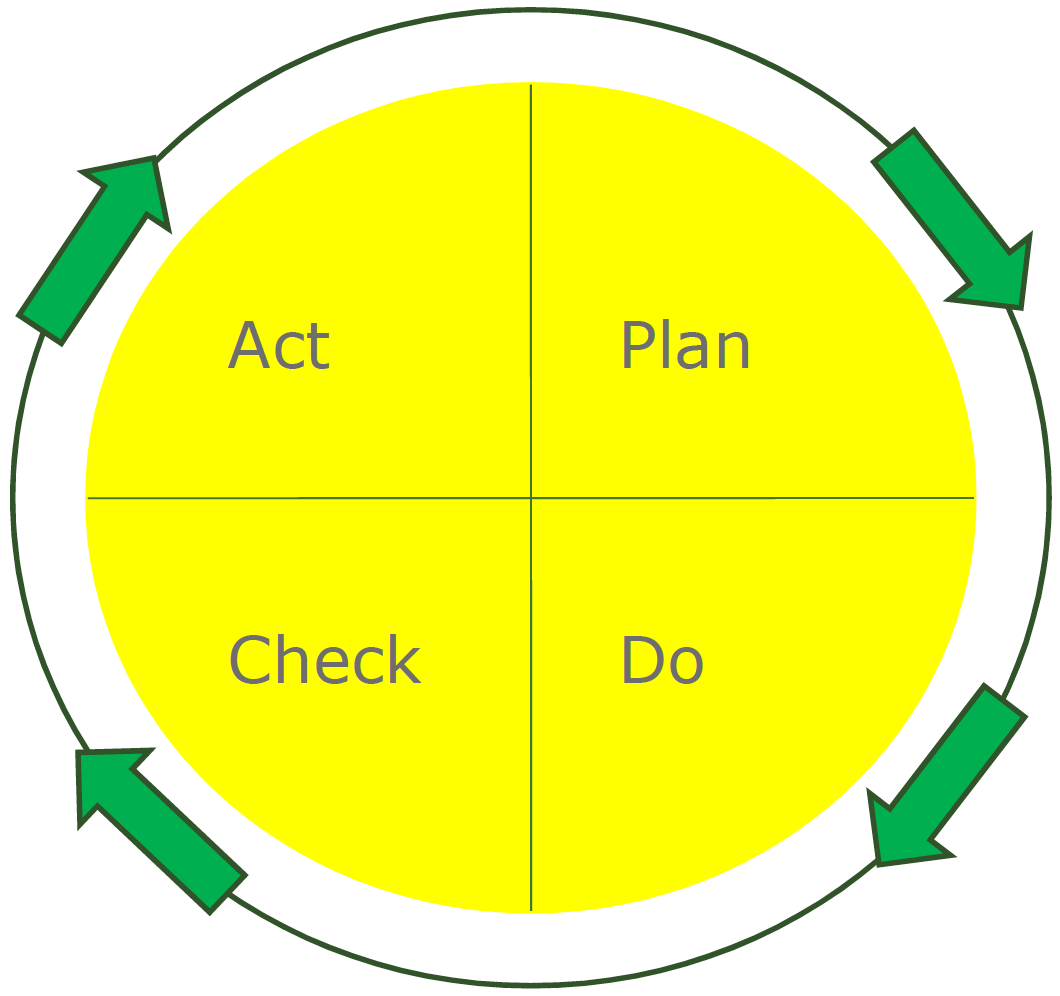
\includegraphics[width=0.4\textwidth]{Figures/DemingCircle.png}
    \caption{A picture of the circular thought behind the Deming Circle}
    \label{fig:demingcircle}
\end{figure}

A more thorough illustration of the four steps can be seen from the following figure \ref{fig:ThoroughDC}.

\begin{figure}
    \centering
    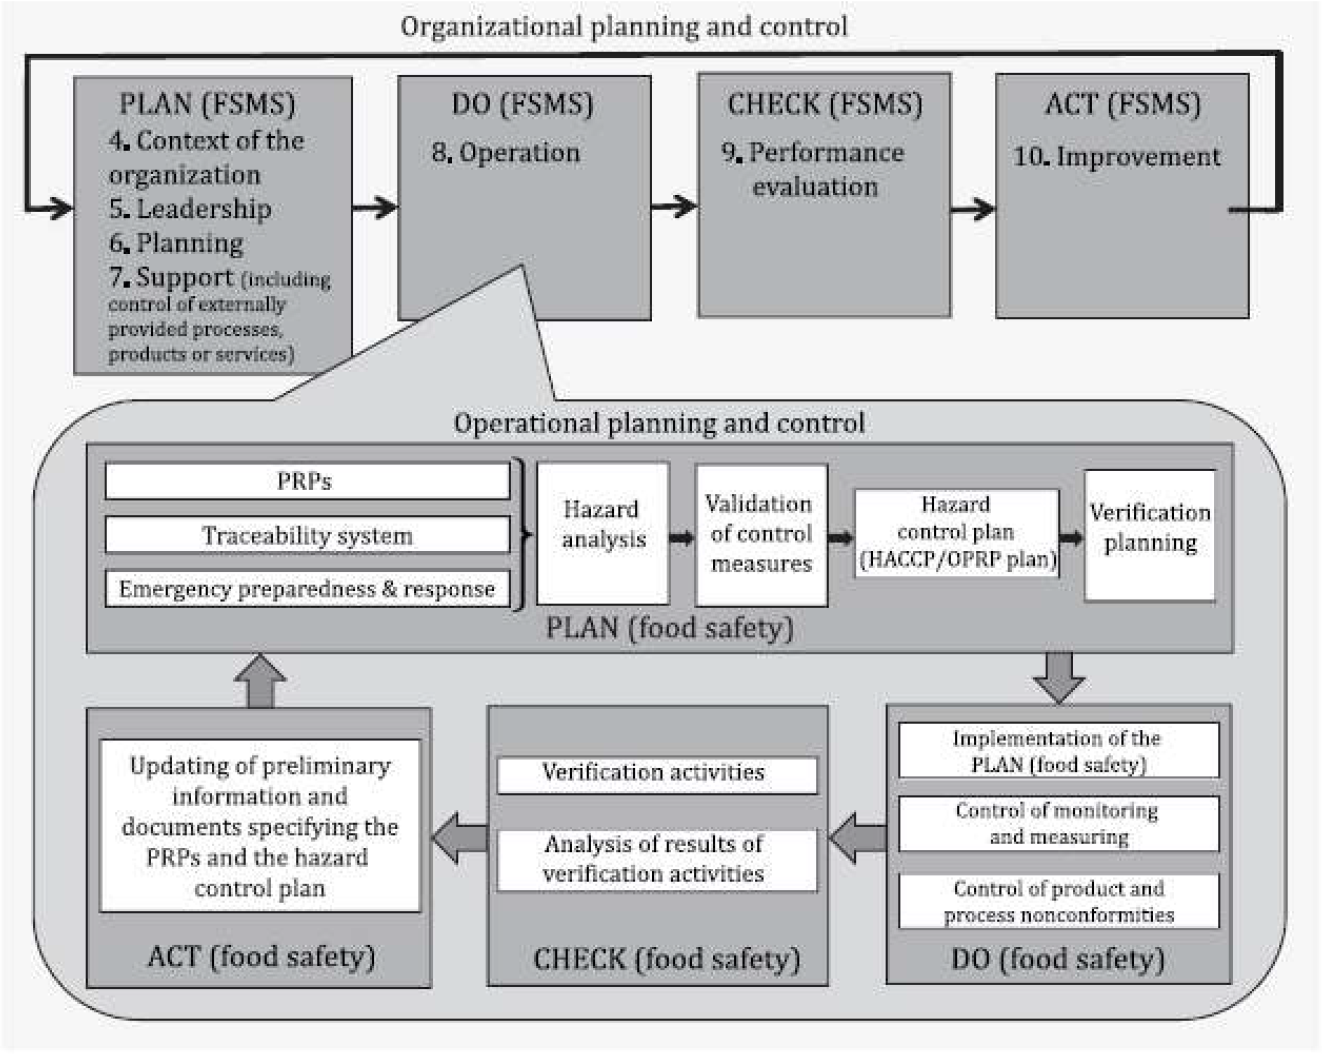
\includegraphics[width=1\textwidth]{Figures/ThoroughDC.png}
    \caption{A thorough illustration of the Plan-Do-Check-Act cycle}
    \label{fig:ThoroughDC}
\end{figure}



\subsection{ISO 22000}
Here are three keypoints of the ISO 22000:

\begin{highlight}
    \begin{itemize}
        \item It combines the prerequisite and operational prerequisite
        programmes (i.e. GMP) and HACCP requirements of Codex
        Alimentarius and quality management requirements of ISO 9000
        \item It reduces confusion about Food Safety Management System
        Standard requirements, since it defines the elements of key
        standards required by leading retailer chains in a single standard
        and defines the Codex HACCP system as the ”standard within the
        standard” to be used
        \item however, the standard is generic, i.e. organizations/companies have to think themselves!
    \end{itemize}
\end{highlight}

There are 10 chapters in the ISO 22000 standard, chapter 4-10 are the main chapters. The first three chapters are the introduction and the scope of the standard. Thus chapters 4-10 are the main chapters of the requirements of the standard.

\begin{highlight}
    \begin{itemize}
        \item Chapter 1: Scope
        \item Chapter 2: Normative references
        \item Chapter 3: Terms and definitions
        \item \textbf{Chapter 4: Context of the organization}
        \item \textbf{Chapter 5: Leadership}
        \item \textbf{Chapter 6: Planning}
        \item \textbf{Chapter 7: Support}
        \item \textbf{Chapter 8: Operation}
        \item \textbf{Chapter 9: Performance evaluation}
        \item \textbf{Chapter 10: Improvement}
    \end{itemize}
\end{highlight}


\section{05.09.24 - HACCP - step 9: monitoring procedures}

HACCP stands for: (H)azard (A)nalysis and (C)ritical (C)ontrol (P)oints
The intention behind this is:

\begin{highlight}
    \begin{itemize}
        \item The internationally recognized procedure to ensure the production of safe foods
        \item Over the last 50 years, HACCP has evolved from
        \item 3 principles to
        \item 7 principles to
        \item 12 steps (incl. the 7 principles)
        \item Codex Alimentarius CAC/RCP 1-1969
    \end{itemize}
\end{highlight}

The HACCP consist of 12 steps (Codex Alimentarius CAC/RCP 1-1969), 5 preliminary steps and 7 principles. The 12 steps are:

\begin{highlight}
    \begin{itemize}
        \item 1 -  Assemble HACCP team
        \item 2 -  Describe product
        \item 3 -  Identify intended use of the product
        \item 4 -  Construct process flow diagram for the product
        \item 5 -  Verification of process flow diagram
        \item 6 -  Conduct a hazard analysis
        \item 7 -  Determine critical control points (CCP’s)
        \item 8 -  Establish critical limits for each CCP
        \item 9 -  Establish monitoring procedures for each CCP
        \item 10 - Establish corrective actions for each CCP
        \item 11 - Establish verification procedures for each CCP
        \item 12 - Establish record keeping and documentation procedures
    \end{itemize}
\end{highlight}

